% -*- TeX -*-
\documentclass[aspectration=169]{beamer}

\usepackage{tikz}
\usetikzlibrary{shapes,arrows,calc}
\usetikzlibrary{decorations.pathreplacing}
\usetikzlibrary{fit,matrix}

\usepackage{listings}
\lstset{basicstyle=\tiny\ttfamily}
\makeatletter
\renewcommand\tiny{\@setfontsize\tiny{5}{6}}
\makeatother

\title{PyLith Modeling Tutorial}
\subtitle{Debugging PyLith v2.1.4 Simulations}
\author{Brad Aagaard \\
  Charles Williams \\
  Matthew Knepley}
\institute{
\includegraphics[scale=0.4]{../../logos/cig_blackfg}}
\date{September 12, 2016}


% ---------------------------------------------------- CUSTOMIZATION
%\renewcommand{\thispdfpagelabel}[1]{}
\newcommand{\component}[1]{{\tt\color{blue}#1}}
\newcommand{\property}[1]{{\it\color{orange}#1}}
\newcommand{\important}[1]{{\color{red}#1}}
\newcommand{\cfg}[1]{{\footnotesize\tt \color{blue}#1}}
\newcommand{\cmd}[1]{{\footnotesize\tt \color{ltred}#1}}
\newcommand{\errlabel}[1]{{\small \color{blue}#1}}
\newcommand{\debuginfo}[1]{{\small \color{green}#1}}

\usetheme{SectionsLogo}

% ========================================================= DOCUMENT
\begin{document}

% ------------------------------------------------------------ SLIDE
\maketitle

% ------------------------------------------------------------ SLIDE
\logo{
\includegraphics[height=4.5ex]{../../logos/cig_blackfg}}

% ========================================================== SECTION
\section{Debugging}
\subsection{Parameters}

% ------------------------------------------------------------ SLIDE
\begin{frame}
  \frametitle{What parameters are available?}
  \summary{Parameters are specified as a hierarchy of components and properties}

  \begin{itemize}
  \item Components (Facilities) are the object building blocks\\
    \important{Appendix B of the PyLith manual lists all of the components}
    \begin{itemize}
    \item Problem \component{TimeDependent}
    \item Boundary conditions \component{DirichletBC}
    \item Faults \component{FaultCohesiveKin}
    \item Materials \component{MaxwellViscoelastic3D}
    \item Output managers \component{OutputSolnSubset}
    \item Readers \component{MeshIOCubit}
    \end{itemize}
  \item Properties are the basic types
    \begin{itemize}
    \item String \property{mat\_viscoelastic.spatialdb}
    \item Integer \property{4}
    \item Float \property{2.3}
    \item Dimensioned quantity \property{2.5*year}
    \item Array of Strings, Integers, or Floats \property{[0, 0, 1]}
    \end{itemize}
  \end{itemize}
  
\end{frame}


% ------------------------------------------------------------ SLIDE
\begin{frame}
  \frametitle{How do I show the values of the current parameters?}
  \summary{Case study: {\tt examples/3d/hex8/step01}}

  \begin{itemize}
  \item All current parameters and their values\\
    \cmd{pylithinfo [--verbose] [-o pylith\_parameters.txt] [-h] [PyLith args]}\\
    \cmd{pylithinfo --verbose step01.cfg}
  \item Components and properties for given component \cmd{--help}
    \begin{description}
    \item[step01.cfg] \cfg{[pylithapp.timedependent.bc.z\_neg]}
    \item[shell] \cmd{pylith step01.cfg --timedependent.bc.z\_neg.help}
    \end{description}
  \item Current components of a given component \cmd{--help-components}
    \begin{description}
    \item[step01.cfg] \cfg{[pylithapp.timedependent.bc.z\_neg]}
    \item[shell] \cmd{pylith step01.cfg --timedependent.bc.z\_neg.help-components}
    \end{description}
  \item Current properties of a given component \cmd{--help-properties}
    \begin{description}
    \item[step01.cfg] \cfg{[pylithapp.timedependent.bc.z\_neg]}
    \item[shell] \cmd{pylith step01.cfg --timedependent.bc.z\_neg.help-properties}
    \end{description}
  \end{itemize}

\end{frame}


% ------------------------------------------------------------ SLIDE
\begin{frame}
  \frametitle{What about a GUI?}
  \summary{Browser-based GUI under development}

  \begin{itemize}
  \item Use web browser as GUI to parameters
    \begin{itemize}
    \item See all parameters with descriptions
    \item See possible choices for components and properties
    \end{itemize}
  \item Basic validation of parameters
  \item Export parameters to single file\\
    Facilitate archiving parameters used in given simulation
  \end{itemize}

  \vfill
  Started in Oct 2013 but v2.0 and v3.0 releases have higher priority
  
\end{frame}


% ========================================================== SECTION
\section{Error Messages}
\subsection{}

% ------------------------------------------------------------ SLIDE
\begin{frame}
  \frametitle{Debugging Examples}
  \summary{See {\tt examples/debugging}}

  \begin{description}
  \item[Step01] Simple shear using Dirichlet BC in static simulation
  \item[Step02] Prescribed fault slip with Dirichlet BC
    \begin{itemize}
    \item Static simulation
    \item Fault is embedded within the domain
    \end{itemize}
  \item[Step03] Spontaneous rupture with Dirichlet BC
    \begin{itemize}
    \item Static simulation
    \item Static friction ($\mu_f=0.6$)
    \item Slip driven by simple shear
    \end{itemize}
  \end{description}
  \vfill
  Correct files are provided for reference
  
\end{frame}


% ========================================================== SECTION
\subsection{Step01}

% ------------------------------------------------------------ SLIDE
\begin{frame}[fragile]
  \frametitle{Step01: Error(s) 1}
  \summary{Error found while doing very basic validation of parameters}

\cmd{\$ pylith step01.cfg}\\
\errlabel{Error message}
\begin{onlyenv}<1>
\begin{lstlisting}
 >> {default}::
 -- pyre.inventory(error)
 -- timedependent.bc.dirichletbc.label <- ''
 -- Label for group/nodeset/pset in mesh not specified.
 >> step01.cfg:59:
 -- pyre.inventory(error)
 -- pylithapp.timedependent.bc.x_posx.bc_dof <- '[1]'
 -- unknown component 'pylithapp.timedependent.bc.x_posx'
 >> step01.cfg:61:
 -- pyre.inventory(error)
 -- pylithapp.timedependent.bc.x_posx.db_initial <- 'spatialdata.spatialdb.UniformDB'
 -- unknown component 'pylithapp.timedependent.bc.x_posx'
 >> step01.cfg:60:
 -- pyre.inventory(error)
 -- pylithapp.timedependent.bc.x_posx.label <- 'face_xpos'
 -- unknown component 'pylithapp.timedependent.bc.x_posx'
 >> step01.cfg:64:
 -- pyre.inventory(error)
 -- pylithapp.timedependent.bc.x_posx.db_initial.data <- '[0.0*m, +1.0*m, 0.0*m]'
 -- unknown component 'pylithapp.timedependent.bc.x_posx.db_initial'
 >> step01.cfg:63:
 -- pyre.inventory(error)
 -- pylithapp.timedependent.bc.x_posx.db_initial.values <- '[displacement-x, displacement-y, displacement-z]'
 -- unknown component 'pylithapp.timedependent.bc.x_posx.db_initial'
 >> step01.cfg:62:
 -- pyre.inventory(error)
 -- pylithapp.timedependent.bc.x_posx.db_initial.label <- 'Dirichlet BC on +x'
 -- unknown component 'pylithapp.timedependent.bc.x_posx.db_initial'
...
\end{lstlisting}
\end{onlyenv}
\begin{onlyenv}<2>
\begin{lstlisting}
...
>> step01.cfg:99:
 -- pyre.inventory(error)
 -- pylithapp.timedependent.implicit.output.outputsoln.write.filename <- 'output/step01.vtk'
 -- unknown component 'pylithapp.timedependent.implicit.output.outputsoln.write'
usage: pylith [--<property>=<value>] [--<facility>.<property>=<value>] [FILE.cfg] ...
component 'pylithapp'
    properties: help, help-components, help-persistence, help-properties, include-citations, initialize-only, job, launcher, mesh_generator, nodes, perf_logger, petsc, problem, scheduler, start-python-debugger, typos, weaver
    facilities: job,launcher,mesh_generator,perf_logger,petsc,problem,scheduler,weaver
For more information:
  --help-properties: prints details about user settable properties
  --help-components: prints details about user settable facilities and components
pylithapp: configuration error(s)
\end{lstlisting}
\end{onlyenv}

  
\end{frame}


% ------------------------------------------------------------ SLIDE
\begin{frame}[fragile]
  \frametitle{Step01: Resolution 1}
  \summary{Error found while doing very basic validation of parameters}

\errlabel{Error message}
\begin{lstlisting}
>> {default}::
-- pyre.inventory(error)
-- timedependent.bc.dirichletbc.label <- ’’
-- Label for group/nodeset/pset in mesh not specified.
>> step01.cfg:59:
-- pyre.inventory(error)
-- pylithapp.timedependent.bc.x_posx.bc_dof <- ’[1]’
-- unknown component ’pylithapp.timedependent.bc.x_posx ’
...
\end{lstlisting}
\errlabel{Component hierarchy}
\begin{lstlisting}
pylithapp.timedependent.bc.x_posx
\end{lstlisting}\pause
\errlabel{Debug:} \debuginfo{Examine parameters for {\tt pylithapp.timedependent.bc}}\pause\\
\errlabel{Resolution}
\begin{lstlisting}
[pylithapp.timedependent.bc.x_pos]
\end{lstlisting}


\end{frame}


% ------------------------------------------------------------ SLIDE
\begin{frame}[fragile]
  \frametitle{Step01: Error 2}
  \summary{Error found in parsing {\tt .cfg} file}

\cmd{\$ pylith step01.cfg}\\
\errlabel{{\tt .cfg} file with line number}
\begin{lstlisting}
 >> step01.cfg:99:
\end{lstlisting}
\errlabel{Error message}
\begin{lstlisting}
 -- pyre.inventory(error)
 -- pylithapp.timedependent.implicit.output.outputsoln.write.filename <- 'output/step01.vtk'
 -- unknown component 'pylithapp.timedependent.implicit.output.outputsoln.write'
\end{lstlisting}
\errlabel{Usage information}
\begin{lstlisting}
usage: pylith [--<property>=<value>] [--<facility>.<property>=<value>] [FILE.cfg] ...
component 'pylithapp'
    properties: help, help-components, help-persistence, help-properties, include-citations, initialize-only, job, launcher, mesh_generator, nodes, perf_logger, petsc, problem, scheduler, start-python-debugger, typos, weaver
    facilities: job,launcher,mesh_generator,perf_logger,petsc,problem,scheduler,weaver
For more information:
  --help-properties: prints details about user settable properties
  --help-components: prints details about user settable facilities and components
pylithapp: configuration error(s)
\end{lstlisting}
  
\end{frame}


% ------------------------------------------------------------ SLIDE
\begin{frame}[fragile]
  \frametitle{Step01: Error 2 Resolution}
  \summary{Error found in parsing {\tt .cfg} file}

\errlabel{Error message}
\begin{lstlisting}
 -- pyre.inventory(error)
 -- pylithapp.timedependent.implicit.output.outputsoln.write.filename <- 'output/step01.vtk'
 -- unknown component 'pylithapp.timedependent.implicit.output.outputsoln.write'
\end{lstlisting}\pause
\errlabel{Debug:} \debuginfo{Look up the properties of the OutputSoln object}\pause\\
\errlabel{Resolution}
\begin{lstlisting}
[pylithapp.problem.formulation.output.domain]
writer.filename = output/step01.vtk
\end{lstlisting}
  
\end{frame}


% ------------------------------------------------------------ SLIDE
\begin{frame}[fragile]
  \frametitle{Step01: Error 3}
  \summary{Error found when initializing integrators}

\cmd{\$ pylith step01.cfg}\\
\errlabel{Python stacktrace}
\begin{lstlisting}
Fatal error. Calling MPI_Abort() to abort PyLith application.
Traceback (most recent call last):
  File "/Volumes/Tools/unix/pylith-dev/clang-3.6.0/lib/python2.7/site-packages/pylith/apps/PetscApplication.py", line 64, in onComputeNodes
    self.main(*args, **kwds)
  File "/Volumes/Tools/unix/pylith-dev/clang-3.6.0/lib/python2.7/site-packages/pylith/apps/PyLithApp.py", line 125, in main
    self.problem.initialize()
  File "/Volumes/Tools/unix/pylith-dev/clang-3.6.0/lib/python2.7/site-packages/pylith/problems/TimeDependent.py", line 120, in initialize
    self.formulation.initialize(self.dimension, self.normalizer)
  File "/Volumes/Tools/unix/pylith-dev/clang-3.6.0/lib/python2.7/site-packages/pylith/problems/Implicit.py", line 121, in initialize
    self._initialize(dimension, normalizer)
  File "/Volumes/Tools/unix/pylith-dev/clang-3.6.0/lib/python2.7/site-packages/pylith/problems/Formulation.py", line 470, in _initialize
    integrator.initialize(totalTime, numTimeSteps, normalizer)
  File "/Volumes/Tools/unix/pylith-dev/clang-3.6.0/lib/python2.7/site-packages/pylith/feassemble/ElasticityImplicit.py", line 56, in initialize
    ModuleElasticityImplicit.initialize(self, self.mesh())
  File "/Volumes/Tools/unix/pylith-dev/clang-3.6.0/lib/python2.7/site-packages/pylith/feassemble/feassemble.py", line 357, in initialize
    def initialize(self, *args): return _feassemble.IntegratorElasticity_initialize(self, *args)
\end{lstlisting}
\errlabel{Error message}
\begin{lstlisting}
RuntimeError: Error occurred while reading spatial database file 'mat_elastic.spatialdb'.
Spatial distribution with data dimensions of 0 cannot have more than one point.
Found 3 points in distribution.
\end{lstlisting}
\errlabel{Abort message}
\begin{lstlisting}
application called MPI_Abort(MPI_COMM_WORLD, -1) - process 0
/Volumes/Tools/unix/cig/clang-3.6.0/bin/nemesis: mpirun: exit 255
/Volumes/Tools/unix/pylith-dev/clang-3.6.0/bin/pylith: /Volumes/Tools/unix/cig/clang-3.6.0/bin/nemesis: exit 1
\end{lstlisting}
  
\end{frame}


% ------------------------------------------------------------ SLIDE
\begin{frame}[fragile]
  \frametitle{Step01: Error 3 Resolution}
  \summary{Error found when initializing integrators}

\errlabel{Error message}
\begin{lstlisting}
RuntimeError: Error occurred while reading spatial database file 'mat_elastic.spatialdb'.
Spatial distribution with data dimensions of 0 cannot have more than one point.
Found 3 points in distribution.
\end{lstlisting}\pause
\errlabel{Debug:} \debuginfo{Look at {\tt mat\_elastic.spatialdb} for errors in data}\pause\\
\errlabel{Resolution}
\begin{lstlisting}
num-locs = 1 // number of locations
\end{lstlisting}
  
\end{frame}


% ------------------------------------------------------------ SLIDE
\begin{frame}[fragile]
  \frametitle{Step01: Error 4}
  \summary{Error found when initializing integrators}

\cmd{\$ pylith step01.cfg}\\
\errlabel{Python stacktrace}
\begin{lstlisting}
Fatal error. Calling MPI_Abort() to abort PyLith application.
Traceback (most recent call last):
  File "/Volumes/Tools/unix/pylith-dev/clang-3.6.0/lib/python2.7/site-packages/pylith/apps/PetscApplication.py", line 64, in onComputeNodes
    self.main(*args, **kwds)
  File "/Volumes/Tools/unix/pylith-dev/clang-3.6.0/lib/python2.7/site-packages/pylith/apps/PyLithApp.py", line 125, in main
    self.problem.initialize()
  File "/Volumes/Tools/unix/pylith-dev/clang-3.6.0/lib/python2.7/site-packages/pylith/problems/TimeDependent.py", line 120, in initialize
    self.formulation.initialize(self.dimension, self.normalizer)
  File "/Volumes/Tools/unix/pylith-dev/clang-3.6.0/lib/python2.7/site-packages/pylith/problems/Implicit.py", line 121, in initialize
    self._initialize(dimension, normalizer)
  File "/Volumes/Tools/unix/pylith-dev/clang-3.6.0/lib/python2.7/site-packages/pylith/problems/Formulation.py", line 470, in _initialize
    integrator.initialize(totalTime, numTimeSteps, normalizer)
  File "/Volumes/Tools/unix/pylith-dev/clang-3.6.0/lib/python2.7/site-packages/pylith/feassemble/ElasticityImplicit.py", line 56, in initialize
    ModuleElasticityImplicit.initialize(self, self.mesh())
  File "/Volumes/Tools/unix/pylith-dev/clang-3.6.0/lib/python2.7/site-packages/pylith/feassemble/feassemble.py", line 357, in initialize
    def initialize(self, *args): return _feassemble.IntegratorElasticity_initialize(self, *args)
\end{lstlisting}
\errlabel{Error message}
\begin{lstlisting}
RuntimeError: Error occurred while reading spatial database file 'mat_elastic.spatialdb'.
Number of dimensions in coordinates of spatial distribution (2) does
not match number of dimensions in coordinate system (3)
\end{lstlisting}
\errlabel{Abort message}
\begin{lstlisting}
application called MPI_Abort(MPI_COMM_WORLD, -1) - process 0
/Volumes/Tools/unix/cig/clang-3.6.0/bin/nemesis: mpirun: exit 255
/Volumes/Tools/unix/pylith-dev/clang-3.6.0/bin/pylith: /Volumes/Tools/unix/cig/clang-3.6.0/bin/nemesis: exit 1
\end{lstlisting}

\end{frame}


% ------------------------------------------------------------ SLIDE
\begin{frame}[fragile]
  \frametitle{Step01: Error 4 Resolution}
  \summary{Error found when initializing integrators}

\errlabel{Error message}
\begin{lstlisting}
RuntimeError: Error occurred while reading spatial database file 'mat_elastic.spatialdb'.
Number of dimensions in coordinates of spatial distribution (2) does
not match number of dimensions in coordinate system (3)
\end{lstlisting}\pause
\errlabel{Debug:} \debuginfo{Look at coordinate system in {\tt mat\_elastic.spatialdb} header}\pause\\
\errlabel{Resolution}
\begin{lstlisting}
space-dim = 3
\end{lstlisting}

\end{frame}


% ------------------------------------------------------------ SLIDE
\begin{frame}[fragile]
  \frametitle{Step01: Error 5}
  \summary{Error found when setting up solution field}

\cmd{\$ pylith step01.cfg}\\
\errlabel{Python stacktrace}
\begin{lstlisting}
Fatal error. Calling MPI_Abort() to abort PyLith application.
Traceback (most recent call last):
  File "/Volumes/Tools/unix/pylith-dev/clang-3.6.0/lib/python2.7/site-packages/pylith/apps/PetscApplication.py", line 64, in onComputeNodes
    self.main(*args, **kwds)
  File "/Volumes/Tools/unix/pylith-dev/clang-3.6.0/lib/python2.7/site-packages/pylith/apps/PyLithApp.py", line 125, in main
    self.problem.initialize()
  File "/Volumes/Tools/unix/pylith-dev/clang-3.6.0/lib/python2.7/site-packages/pylith/problems/TimeDependent.py", line 120, in initialize
    self.formulation.initialize(self.dimension, self.normalizer)
  File "/Volumes/Tools/unix/pylith-dev/clang-3.6.0/lib/python2.7/site-packages/pylith/problems/Implicit.py", line 121, in initialize
    self._initialize(dimension, normalizer)
  File "/Volumes/Tools/unix/pylith-dev/clang-3.6.0/lib/python2.7/site-packages/pylith/problems/Formulation.py", line 516, in _initialize
    constraint.setConstraintSizes(solution)
  File "/Volumes/Tools/unix/pylith-dev/clang-3.6.0/lib/python2.7/site-packages/pylith/bc/bc.py", line 218, in setConstraintSizes
    def setConstraintSizes(self, *args): return
_bc.DirichletBC_setConstraintSizes(self, *args)
\end{lstlisting}
\errlabel{Error message}
\begin{lstlisting}
RuntimeError: Found overly constrained point while setting up constraints for DirichletBC boundary condition 'face_zneg'. Number of DOF at point 503 is 3 and number of attempted constraints is 4.
\end{lstlisting}
\errlabel{Abort information}
\begin{lstlisting}
application called MPI_Abort(MPI_COMM_WORLD, -1) - process 0
/Volumes/Tools/unix/cig/clang-3.6.0/bin/nemesis: mpirun: exit 255
/Volumes/Tools/unix/pylith-dev/clang-3.6.0/bin/pylith: /Volumes/Tools/unix/cig/clang-3.6.0/bin/nemesis: exit 1
\end{lstlisting}
  
\end{frame}


% ------------------------------------------------------------ SLIDE
\begin{frame}[fragile]
  \frametitle{Step01: Error 5 Resolution}
  \summary{Error found when setting up solution field}

\errlabel{Error message}
\begin{lstlisting}
RuntimeError: Found overly constrained point while setting up constraints for DirichletBC boundary condition 'face_zneg'. Number of DOF at point 503 is 3 and number of attempted constraints is 4.
\end{lstlisting}\pause
\errlabel{Debug:} \debuginfo{Look at overlap of constraints in Dirichlet BC}\pause\\
\errlabel{Resolution}
\begin{lstlisting}
[pylithapp.timedependent.bc.y_pos]
bc_dof = [0]
...
[pylithapp.timedependent.bc.y_neg]
bc_dof = [0]
\end{lstlisting}

\end{frame}


% ========================================================== SECTION
\subsection{Step02}

% ------------------------------------------------------------ SLIDE
\begin{frame}[fragile]
  \frametitle{Step02: Error 1}
  \summary{Error found in parsing {\tt .cfg} file}

\cmd{\$ pylith step02.cfg}\\
\errlabel{Configuration error}
\begin{lstlisting}
 >> step02.cfg:30:
 -- pyre.inventory(error)
 -- timedependent.nondimelasticquasistatic.relaxation_time <- '2.0*years'
 -- name 'years' is not defined
pylithapp: configuration error(s)
\end{lstlisting}
  
\end{frame}


% ------------------------------------------------------------ SLIDE
\begin{frame}[fragile]
  \frametitle{Step02: Error 1 Resolution}
  \summary{Error found in parsing {\tt .cfg} file}

\errlabel{Error message}
\begin{lstlisting}
 >> step02.cfg:30:
 -- pyre.inventory(error)
 -- timedependent.nondimelasticquasistatic.relaxation_time <- '2.0*years'
 -- name 'years' is not defined
pylithapp: configuration error(s)
\end{lstlisting}\pause
\errlabel{Debug:} \debuginfo{Pyre is poorly documented. Look for example. :(}\pause\\
\cmd{\$ python}
\begin{lstlisting}
>>> from pyre.units.time import *
>>> dir()
['__builtins__', '__doc__', '__name__', '__package__', 'day', 'hour', 'micro', 'microsecond',
 'milli', 'millisecond', 'minute', 'ms', 'nano', 'nanosecond', 'ns', 'pico',
 'picosecond', 'ps', 's', 'second', 'us', 'year']
\end{lstlisting}
\errlabel{Resolution}
\begin{lstlisting}
relaxation_time = 2.0*year
\end{lstlisting}

\end{frame}


% ------------------------------------------------------------ SLIDE
\begin{frame}[fragile]
  \frametitle{Step02: Error 2}
  \summary{Error doing some basic validation of input}

\cmd{\$ pylith step02.cfg}\\
\errlabel{Python stacktrace}
\begin{lstlisting}
Fatal error. Calling MPI_Abort() to abort PyLith application.
Traceback (most recent call last):
  File "/Volumes/Tools/unix/pylith-dev/clang-3.6.0/lib/python2.7/site-packages/pylith/apps/PetscApplication.py", line 64, in onComputeNodes
    self.main(*args, **kwds)
  File "/Volumes/Tools/unix/pylith-dev/clang-3.6.0/lib/python2.7/site-packages/pylith/apps/PyLithApp.py", line 123, in main
    self.problem.verifyConfiguration()
  File "/Volumes/Tools/unix/pylith-dev/clang-3.6.0/lib/python2.7/site-packages/pylith/problems/TimeDependent.py", line 105, in verifyConfiguration
    self.formulation.verifyConfiguration()
  File "/Volumes/Tools/unix/pylith-dev/clang-3.6.0/lib/python2.7/site-packages/pylith/problems/Formulation.py", line 180, in verifyConfiguration
    integrator.verifyConfiguration()
  File "/Volumes/Tools/unix/pylith-dev/clang-3.6.0/lib/python2.7/site-packages/pylith/faults/FaultCohesiveKin.py", line 140, in verifyConfiguration
    ModuleFaultCohesiveKin.verifyConfiguration(self, self.mesh())
  File "/Volumes/Tools/unix/pylith-dev/clang-3.6.0/lib/python2.7/site-packages/pylith/faults/faults.py", line 365, in verifyConfiguration
    def verifyConfiguration(self, *args): return _faults.FaultCohesiveLagrange_verifyConfiguration(self, *args)
\end{lstlisting}
\errlabel{Error message}
\begin{lstlisting}
RuntimeError: Quadrature is incompatible with cell for fault 'fault_ext'. Cell 256 has 4 edges but quadrature reference cell has 3 edges.
\end{lstlisting}
\errlabel{Abort info}
\begin{lstlisting}
application called MPI_Abort(MPI_COMM_WORLD, -1) - process 0
/Volumes/Tools/unix/cig/clang-3.6.0/bin/nemesis: mpirun: exit 255
/Volumes/Tools/unix/pylith-dev/clang-3.6.0/bin/pylith: /Volumes/Tools/unix/cig/clang-3.6.0/bin/nemesis: exit 1
\end{lstlisting}
  
\end{frame}


% ------------------------------------------------------------ SLIDE
\begin{frame}[fragile]
  \frametitle{Step02: Error 2 Resolution}
  \summary{Error doing some basic validation of input}

\errlabel{Error message}
\begin{lstlisting}
RuntimeError: Quadrature is incompatible with cell for fault 'fault_ext'. Cell 256 has 4 edges but quadrature reference cell has 3 edges.
\end{lstlisting}\pause
\errlabel{Debug:} \debuginfo{Turn on journal for quadrature}\\
\cmd{\$ pylith step02.cfg --problem.interfaces.fault.quadrature.help-components}
\begin{lstlisting}
facilities of 'quadrature':
    cell=<component name>: Reference cell with basis fns and quadrature rules.
        current value: 'fiatsimplex', from {default}
        configurable as: fiatsimplex, cell
\end{lstlisting}\pause
\begin{lstlisting}
[pylithapp.journal.info]
fiatlagrange = 1
fiatsimplex = 1
\end{lstlisting}
\errlabel{Resolution}
\begin{lstlisting}
[pylithapp.timedependent.interfaces.fault]
quadrature.cell = pylith.feassemble.FIATLagrange
\end{lstlisting}

\end{frame}


% ------------------------------------------------------------ SLIDE
\begin{frame}[fragile]
  \frametitle{Step02: Error 3}
  \summary{Error found when initializing integrators}

\cmd{\$ pylith step02.cfg}\\
\errlabel{Python stacktrace}
\begin{lstlisting}
Fatal error. Calling MPI_Abort() to abort PyLith application.
Traceback (most recent call last):
  File "/Volumes/Tools/unix/pylith-dev/clang-3.6.0/lib/python2.7/site-packages/pylith/apps/PetscApplication.py", line 64, in onComputeNodes
    self.main(*args, **kwds)
  File "/Volumes/Tools/unix/pylith-dev/clang-3.6.0/lib/python2.7/site-packages/pylith/apps/PyLithApp.py", line 125, in main
    self.problem.initialize()
  File "/Volumes/Tools/unix/pylith-dev/clang-3.6.0/lib/python2.7/site-packages/pylith/problems/TimeDependent.py", line 120, in initialize
    self.formulation.initialize(self.dimension, self.normalizer)
  File "/Volumes/Tools/unix/pylith-dev/clang-3.6.0/lib/python2.7/site-packages/pylith/problems/Implicit.py", line 121, in initialize
    self._initialize(dimension, normalizer)
  File "/Volumes/Tools/unix/pylith-dev/clang-3.6.0/lib/python2.7/site-packages/pylith/problems/Formulation.py", line 470, in _initialize
    integrator.initialize(totalTime, numTimeSteps, normalizer)
  File "/Volumes/Tools/unix/pylith-dev/clang-3.6.0/lib/python2.7/site-packages/pylith/feassemble/ElasticityImplicit.py", line 56, in initialize
    ModuleElasticityImplicit.initialize(self, self.mesh())
  File "/Volumes/Tools/unix/pylith-dev/clang-3.6.0/lib/python2.7/site-packages/pylith/feassemble/feassemble.py", line 357, in initialize
    def initialize(self, *args): return _feassemble.IntegratorElasticity_initialize(self, *args)
\end{lstlisting}
\errlabel{Error message}
\begin{lstlisting}
RuntimeError: Determinant of Jacobian (1.25e-07) for cell 0 is smaller than minimum permissible value (1e-06)!
The two most likely causes of this are highly distorted cells and nondimensionalization with a length scale that is much larger than the dimensions of the cells.
\end{lstlisting}
\errlabel{Abort info}
\begin{lstlisting}
application called MPI_Abort(MPI_COMM_WORLD, -1) - process 0
/Volumes/Tools/unix/cig/clang-3.6.0/bin/nemesis: mpirun: exit 255
/Volumes/Tools/unix/pylith-dev/clang-3.6.0/bin/pylith: /Volumes/Tools/unix/cig/clang-3.6.0/bin/nemesis: exit 1
\end{lstlisting}
  
\end{frame}


% ------------------------------------------------------------ SLIDE
\begin{frame}[fragile]
  \frametitle{Step02: Error 3 Resolution}
  \summary{Error found when initializing integrators}

\errlabel{Error message}
\begin{lstlisting}
RuntimeError: Determinant of Jacobian (1.25e-07) for cell 0 is smaller than minimum permissible value (1e-06)!
The two most likely causes of this are highly distorted cells and nondimensionalization with a length scale that is much larger than the dimensions of the cells.
\end{lstlisting}\pause
\errlabel{Debug:} \debuginfo{Look at nondimensional scales relative to the parameters}\\
\cmd{\$ pylith step02.cfg --problem.normalizer.help-properties}
\begin{lstlisting}
    length_scale=<dimensional>: Value to nondimensionalize length scale.
        default value: 1000*m
        current value: 1e+06*m, from {file='step02.cfg', line=28, column=-1}
        validator: (greater than 0*m)
    relaxation_time=<dimensional>: Relaxation time to nondimensionalize time.
        default value: 3.15576e+07*s
        current value: 6.31152e+07*s, from {file='step02.cfg', line=30, column=-1}
        validator: (greater than 0*s)
    shear_modulus=<dimensional>: Shear modulus to nondimensionalize pressure.
        default value: 3e+10*m**-1*kg*s**-2
        current value: 3e+10*m**-1*kg*s**-2, from {file='step02.cfg', line=29, column=-1}
        validator: (greater than 0*m**-1*kg*s**-2)
\end{lstlisting}\pause
\errlabel{Resolution}
\begin{lstlisting}
[pylithapp.problem.normalizer]
length_scale = 1.0*km
\end{lstlisting}

\end{frame}


% ------------------------------------------------------------ SLIDE
\begin{frame}[fragile]
  \frametitle{Step02: Error 4}
  \summary{Error found when initializing fault}

\cmd{\$ pylith step02.cfg}\\
\errlabel{Python stacktrace}
\begin{lstlisting}
Fatal error. Calling MPI_Abort() to abort PyLith application.
Traceback (most recent call last):
  File "/Volumes/Tools/unix/pylith-dev/clang-3.6.0/lib/python2.7/site-packages/pylith/apps/PetscApplication.py", line 64, in onComputeNodes
    self.main(*args, **kwds)
  File "/Volumes/Tools/unix/pylith-dev/clang-3.6.0/lib/python2.7/site-packages/pylith/apps/PyLithApp.py", line 125, in main
    self.problem.initialize()
  File "/Volumes/Tools/unix/pylith-dev/clang-3.6.0/lib/python2.7/site-packages/pylith/problems/TimeDependent.py", line 120, in initialize
    self.formulation.initialize(self.dimension, self.normalizer)
  File "/Volumes/Tools/unix/pylith-dev/clang-3.6.0/lib/python2.7/site-packages/pylith/problems/Implicit.py", line 121, in initialize
    self._initialize(dimension, normalizer)
  File "/Volumes/Tools/unix/pylith-dev/clang-3.6.0/lib/python2.7/site-packages/pylith/problems/Formulation.py", line 470, in _initialize
    integrator.initialize(totalTime, numTimeSteps, normalizer)
  File "/Volumes/Tools/unix/pylith-dev/clang-3.6.0/lib/python2.7/site-packages/pylith/faults/FaultCohesiveKin.py", line 166, in initialize
    FaultCohesive.initialize(self, totalTime, numTimeSteps, normalizer)
  File "/Volumes/Tools/unix/pylith-dev/clang-3.6.0/lib/python2.7/site-packages/pylith/faults/Fault.py", line 170, in initialize
    ModuleFault.initialize(self, self.mesh(), self.upDir)
  File "/Volumes/Tools/unix/pylith-dev/clang-3.6.0/lib/python2.7/site-packages/pylith/faults/faults.py", line 321, in initialize
    def initialize(self, *args): return _faults.Fault_initialize(self, *args)
\end{lstlisting}
\errlabel{Error message}
\begin{lstlisting}
RuntimeError: Could not find value left-lateral-slip in spatial database
Final slip. Available values are:
  lateral-slip
  reverse-slip
  fault-opening
\end{lstlisting}
\errlabel{Abort message}
\begin{lstlisting}
application called MPI_Abort(MPI_COMM_WORLD, -1) - process 0
/Volumes/Tools/unix/cig/clang-3.6.0/bin/nemesis: mpirun: exit 255
/Volumes/Tools/unix/pylith-dev/clang-3.6.0/bin/pylith: /Volumes/Tools/unix/cig/clang-3.6.0/bin/nemesis: exit 1
\end{lstlisting}

\end{frame}


% ------------------------------------------------------------ SLIDE
\begin{frame}[fragile]
  \frametitle{Step02: Error 4 Resolution}
  \summary{Error found when initializing fault}

\errlabel{Error message}
\begin{lstlisting}
RuntimeError: Could not find value left-lateral-slip in spatial database
Final slip. Available values are:
  lateral-slip
  reverse-slip
  fault-opening
\end{lstlisting}\pause
\errlabel{Resolution}
\begin{lstlisting}
slip.values = [left-lateral-slip, reverse-slip, fault-opening]
\end{lstlisting}

\end{frame}


% ------------------------------------------------------------ SLIDE
\begin{frame}[fragile]
  \frametitle{Step02: Error 5}
  \summary{Error found when setting up solution field}

\cmd{\$ pylith step02.cfg}\\
\errlabel{Python stacktrace}
\begin{lstlisting}
Fatal error. Calling MPI_Abort() to abort PyLith application.
Traceback (most recent call last):
  File "/Volumes/Tools/unix/pylith-dev/gcc-4.7.3/lib/python2.7/site-packages/pylith/apps/PetscApplication.py", line 64, in onComputeNodes
    self.main(*args, **kwds)
  File "/Volumes/Tools/unix/pylith-dev/gcc-4.7.3/lib/python2.7/site-packages/pylith/apps/PyLithApp.py", line 125, in main
    self.problem.initialize()
  File "/Volumes/Tools/unix/pylith-dev/gcc-4.7.3/lib/python2.7/site-packages/pylith/problems/TimeDependent.py", line 119, in initialize
    self.formulation.initialize(self.dimension, self.normalizer)
  File "/Volumes/Tools/unix/pylith-dev/gcc-4.7.3/lib/python2.7/site-packages/pylith/problems/Implicit.py", line 122, in initialize
    self._initialize(dimension, normalizer)
  File "/Volumes/Tools/unix/pylith-dev/gcc-4.7.3/lib/python2.7/site-packages/pylith/problems/Formulation.py", line 522, in _initialize
    integrator.checkConstraints(solution)
  File "/Volumes/Tools/unix/pylith-dev/gcc-4.7.3/lib/python2.7/site-packages/pylith/faults/faults.py", line 366, in checkConstraints
    def checkConstraints(self, *args): return _faults.FaultCohesiveLagrange_checkConstraints(self, *args)
\end{lstlisting}
\errlabel{Error message}
\begin{lstlisting}
RuntimeError: Vertex with label '396' on negative side of fault 'fault_ext' is constrained.
Fault vertices cannot be constrained.
\end{lstlisting}
\errlabel{Abort info}
\begin{lstlisting}
application called MPI_Abort(MPI_COMM_WORLD, -1) - process 0
/Volumes/Tools/unix/cig/gcc-4.7.3/bin/nemesis: mpirun: exit 255
/Volumes/Tools/unix/pylith-dev/gcc-4.7.3/bin/pylith: /Volumes/Tools/unix/cig/gcc-4.7.3/bin/nemesis: exit 1
\end{lstlisting}

\end{frame}


% ------------------------------------------------------------ SLIDE
\begin{frame}[fragile]
  \frametitle{Step02: Error 5 Resolution}
  \summary{Error found when setting up solution field}

\errlabel{Error message}
\begin{lstlisting}
RuntimeError: Vertex with label '396' on negative side of fault 'fault_ext' is constrained.
Fault vertices cannot be constrained.
\end{lstlisting}\pause
\errlabel{Debug:} \debuginfo{Oops. Didn't mean to use through-going fault!}\pause\\
\errlabel{Resolution}
\begin{lstlisting}
[pylithapp.timedependent.interfaces.fault]
label = fault
\end{lstlisting}

\end{frame}


% ------------------------------------------------------------ SLIDE
\begin{frame}[fragile]
  \frametitle{Step02: Error 6}
  \summary{Error when initializing fault}

\cmd{\$ pylith step02.cfg}\\
\errlabel{Python stacktrace}
\begin{lstlisting}
Fatal error. Calling MPI_Abort() to abort PyLith application.
Traceback (most recent call last):
  File "/Volumes/Tools/unix/pylith-dev/clang-3.6.0/lib/python2.7/site-packages/pylith/apps/PetscApplication.py", line 64, in onComputeNodes
    self.main(*args, **kwds)
  File "/Volumes/Tools/unix/pylith-dev/clang-3.6.0/lib/python2.7/site-packages/pylith/apps/PyLithApp.py", line 125, in main
    self.problem.initialize()
  File "/Volumes/Tools/unix/pylith-dev/clang-3.6.0/lib/python2.7/site-packages/pylith/problems/TimeDependent.py", line 120, in initialize
    self.formulation.initialize(self.dimension, self.normalizer)
  File "/Volumes/Tools/unix/pylith-dev/clang-3.6.0/lib/python2.7/site-packages/pylith/problems/Implicit.py", line 121, in initialize
    self._initialize(dimension, normalizer)
  File "/Volumes/Tools/unix/pylith-dev/clang-3.6.0/lib/python2.7/site-packages/pylith/problems/Formulation.py", line 470, in _initialize
    integrator.initialize(totalTime, numTimeSteps, normalizer)
  File "/Volumes/Tools/unix/pylith-dev/clang-3.6.0/lib/python2.7/site-packages/pylith/faults/FaultCohesiveKin.py", line 166, in initialize
    FaultCohesive.initialize(self, totalTime, numTimeSteps, normalizer)
  File "/Volumes/Tools/unix/pylith-dev/clang-3.6.0/lib/python2.7/site-packages/pylith/faults/Fault.py", line 170, in initialize
    ModuleFault.initialize(self, self.mesh(), self.upDir)
  File "/Volumes/Tools/unix/pylith-dev/clang-3.6.0/lib/python2.7/site-packages/pylith/faults/faults.py", line 321, in initialize
    def initialize(self, *args): return _faults.Fault_initialize(self, *args)
\end{lstlisting}
\errlabel{Error message}
\begin{lstlisting}
RuntimeError: Error computing orientation of cell face. Cannot resolve tangential components into unambigious directions.
Up direction (0, 0, 1)  cannot be parallel to the face normal (0, 0, 1).
If the face is horizontal, adjust the up_dir parameter.
\end{lstlisting}
\errlabel{Abort info}
\begin{lstlisting}
application called MPI_Abort(MPI_COMM_WORLD, -1) - process 0
/Volumes/Tools/unix/cig/clang-3.6.0/bin/nemesis: mpirun: exit 255
/Volumes/Tools/unix/pylith-dev/clang-3.6.0/bin/pylith: /Volumes/Tools/unix/cig/clang-3.6.0/bin/nemesis: exit 1
\end{lstlisting}

\end{frame}


% ------------------------------------------------------------ SLIDE
\begin{frame}[fragile]
  \frametitle{Step02: Error 6 Resolution}
  \summary{Error found when initializing fault}

\errlabel{Error message}
\begin{lstlisting}
RuntimeError: Error computing orientation of cell face. Cannot resolve tangential components into unambigious directions.
Up direction (0, 0, 1)  cannot be parallel to the face normal (0, 0, 1).
If the face is horizontal, adjust the up_dir parameter.
\end{lstlisting}\pause
\errlabel{Debug:} \debuginfo{Change up-dir}
\begin{lstlisting}
up_dir = [1,0,1]
\end{lstlisting}\pause
\errlabel{Debug:} \debuginfo{Look at fault surface}\pause\\
\errlabel{Resolution:} \debuginfo{Mark buried edges}
\begin{lstlisting}
[pylithapp.timedependent.interfaces.fault]
label = fault
edge = fault_edge
up_dir = [0,0,1]
\end{lstlisting}

\end{frame}


% ========================================================== SECTION
\subsection{Fault Edges}

% ------------------------------------------------------------ SLIDE
\begin{frame}
  \frametitle{Insertion of Cohesive Cells}
  \summary{}

  \begin{center}
    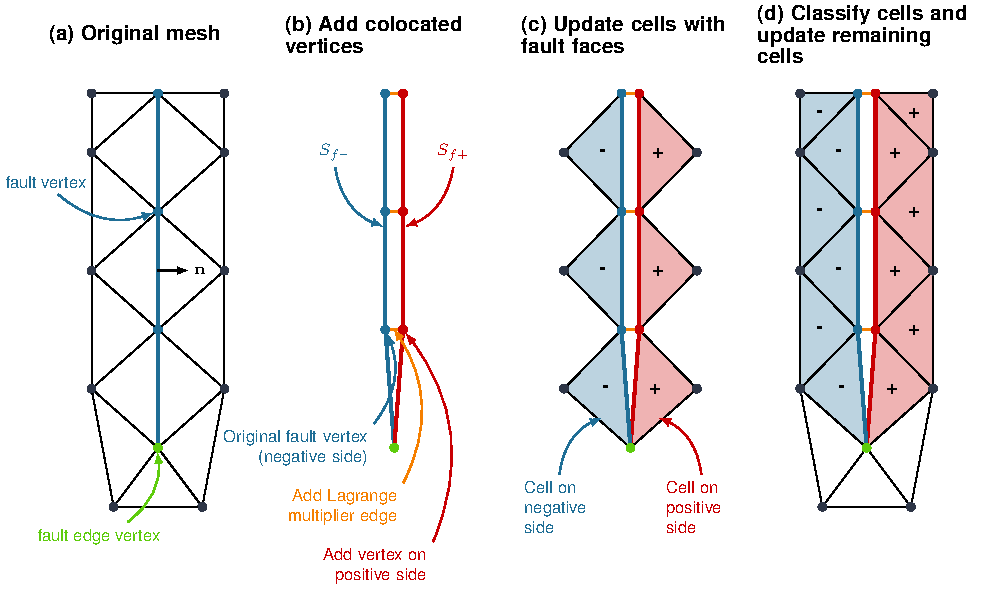
\includegraphics[height=7.0cm]{figs/cohesivecells}
  \end{center}

\end{frame}


% ------------------------------------------------------------ SLIDE
\begin{frame}
  \frametitle{Forgetting to Mark Buried Edges}
  \summary{PyLith will extend the fault one cell in an arbitrary fashion}

  Purple region shows intended fault surface.
  \begin{center}
    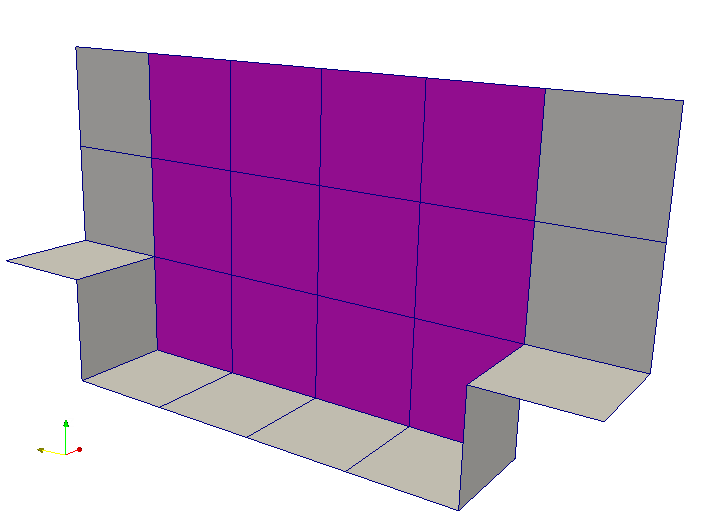
\includegraphics[height=7.2cm]{figs/faultedges}
  \end{center}
  
\end{frame}


% ========================================================== SECTION
\subsection{Step03}

% ------------------------------------------------------------ SLIDE
\begin{frame}[fragile]
  \frametitle{Step03: Error 1}
  \summary{Error doing basic validation on parameters}

\cmd{\$ pylith step02.cfg}\\
\errlabel{Python stacktrace}
\begin{lstlisting}
Fatal error. Calling MPI_Abort() to abort PyLith application.
Traceback (most recent call last):
  File "/Volumes/Tools/unix/pylith-dev/gcc-4.7.3/lib/python2.7/site-packages/pylith/apps/PetscApplication.py", line 64, in onComputeNodes
    self.main(*args, **kwds)
  ...
  File "/Volumes/Tools/unix/pylith-dev/gcc-4.7.3/lib/python2.7/site-packages/pylith/faults/FaultCohesiveDyn.py", line 145, in verifyConfiguration
    FaultCohesive.verifyConfiguration(self)
  File "/Volumes/Tools/unix/pylith-dev/gcc-4.7.3/lib/python2.7/site-packages/pylith/faults/Fault.py", line 156, in verifyConfiguration
    self.output.verifyConfiguration(self.mesh())
  File "/Volumes/Tools/unix/pylith-dev/gcc-4.7.3/lib/python2.7/site-packages/pylith/meshio/OutputManager.py", line 128, in verifyConfiguration
    self._verifyFields(self.dataProvider().availableFields)
  File "/Volumes/Tools/unix/pylith-dev/gcc-4.7.3/lib/python2.7/site-packages/pylith/meshio/OutputManager.py", line 383, in _verifyFields
    raise ValueError(msg)
\end{lstlisting}
\errlabel{Error message}
\begin{lstlisting}
ValueError: Requested fields not available for output.
Data provider: 'faultcohesivedyn'
Field type: 'vertex'
Data type: 'data'
Available fields:  'slip' 'slip_rate' 'traction'
Fields not available:  'initial_traction'
\end{lstlisting}
\errlabel{Abort info}
\begin{lstlisting}
application called MPI_Abort(MPI_COMM_WORLD, -1) - process 0
/Volumes/Tools/unix/cig/gcc-4.7.3/bin/nemesis: mpirun: exit 255
\end{lstlisting}

\end{frame}


% ------------------------------------------------------------ SLIDE
\begin{frame}[fragile]
  \frametitle{Step03: Error 1 Resolution}
  \summary{Error doing basic validation on parameters}

\errlabel{Error message}
\begin{lstlisting}
ValueError: Requested fields not available for output.
Data provider: 'faultcohesivedyn'
Field type: 'vertex'
Data type: 'data'
Available fields:  'slip' 'slip_rate' 'traction'
Fields not available:  'initial_traction'
\end{lstlisting}\pause
\errlabel{Resolution}
\begin{lstlisting}
vertex_data_fields = [slip,slip_rate,traction]
\end{lstlisting}

\end{frame}


% ------------------------------------------------------------ SLIDE
\begin{frame}[fragile]
  \frametitle{Step03: Error 2}
  \summary{Error creating solution field}

\cmd{\$ pylith step03.cfg}\\
\errlabel{Python stacktrace}
\begin{lstlisting}
Fatal error. Calling MPI_Abort() to abort PyLith application.
Traceback (most recent call last):
  File "/Volumes/Tools/unix/pylith-dev/gcc-4.7.3/lib/python2.7/site-packages/pylith/apps/PetscApplication.py", line 64, in onComputeNodes
    self.main(*args, **kwds)
  File "/Volumes/Tools/unix/pylith-dev/gcc-4.7.3/lib/python2.7/site-packages/pylith/apps/PyLithApp.py", line 125, in main
    self.problem.initialize()
  File "/Volumes/Tools/unix/pylith-dev/gcc-4.7.3/lib/python2.7/site-packages/pylith/problems/TimeDependent.py", line 119, in initialize
    self.formulation.initialize(self.dimension, self.normalizer)
  File "/Volumes/Tools/unix/pylith-dev/gcc-4.7.3/lib/python2.7/site-packages/pylith/problems/Implicit.py", line 122, in initialize
    self._initialize(dimension, normalizer)
  File "/Volumes/Tools/unix/pylith-dev/gcc-4.7.3/lib/python2.7/site-packages/pylith/problems/Formulation.py", line 516, in _initialize
    constraint.setConstraintSizes(solution)
  File "/Volumes/Tools/unix/pylith-dev/gcc-4.7.3/lib/python2.7/site-packages/pylith/bc/bc.py", line 218, in setConstraintSizes
    def setConstraintSizes(self, *args): return _bc.DirichletBC_setConstraintSizes(self, *args)
\end{lstlisting}
\errlabel{Error message}
\begin{lstlisting}
RuntimeError: Found overly constrained point while setting up constraints for DirichletBC
boundary condition 'face_zneg'. Number of DOF at point 535 is 3 and number of attempted
constraints is 4.
\end{lstlisting}
\errlabel{Abort info}
\begin{lstlisting}
application called MPI_Abort(MPI_COMM_WORLD, -1) - process 0
/Volumes/Tools/unix/cig/gcc-4.7.3/bin/nemesis: mpirun: exit 255
/Volumes/Tools/unix/pylith-dev/gcc-4.7.3/bin/pylith:
/Volumes/Tools/unix/cig/gcc-4.7.3/bin/nemesis: exit 1
\end{lstlisting}

\end{frame}


% ------------------------------------------------------------ SLIDE
\begin{frame}[fragile]
  \frametitle{Step03: Error 2 Resolution}
  \summary{Error creating solution field}

\errlabel{Error message}
\begin{lstlisting}
RuntimeError: Found overly constrained point while setting up constraints for DirichletBC
boundary condition 'face_zneg'. Number of DOF at point 535 is 3 and number of attempted
constraints is 4.
\end{lstlisting}\pause
\errlabel{Debug:} \debuginfo{Look for overlap of constraints in Dirichlet BC}\pause\\
\errlabel{Resolution}
\begin{lstlisting}
[pylithapp.timedependent.bc.x_pos]
bc_dof = [0, 1]
...
[pylithapp.timedependent.bc.x_neg]
bc_dof = [0, 1]
\end{lstlisting}

\end{frame}


% ------------------------------------------------------------ SLIDE
\begin{frame}[fragile]
  \frametitle{Step03: Error 3}
  \summary{Error creating solution field}

\cmd{\$ pylith step03.cfg}\\
\errlabel{Python stacktrace}
\begin{lstlisting}
Fatal error. Calling MPI_Abort() to abort PyLith application.
Traceback (most recent call last):
  File "/Volumes/Tools/unix/pylith-dev/gcc-4.7.3/lib/python2.7/site-packages/pylith/apps/PetscApplication.py", line 64, in onComputeNodes
    self.main(*args, **kwds)
  File "/Volumes/Tools/unix/pylith-dev/gcc-4.7.3/lib/python2.7/site-packages/pylith/apps/PyLithApp.py", line 125, in main
    self.problem.initialize()
  File "/Volumes/Tools/unix/pylith-dev/gcc-4.7.3/lib/python2.7/site-packages/pylith/problems/TimeDependent.py", line 119, in initialize
    self.formulation.initialize(self.dimension, self.normalizer)
  File "/Volumes/Tools/unix/pylith-dev/gcc-4.7.3/lib/python2.7/site-packages/pylith/problems/Implicit.py", line 122, in initialize
    self._initialize(dimension, normalizer)
  File "/Volumes/Tools/unix/pylith-dev/gcc-4.7.3/lib/python2.7/site-packages/pylith/problems/Formulation.py", line 522, in _initialize
    integrator.checkConstraints(solution)
  File "/Volumes/Tools/unix/pylith-dev/gcc-4.7.3/lib/python2.7/site-packages/pylith/faults/faults.py", line 366, in checkConstraints
    def checkConstraints(self, *args): return _faults.FaultCohesiveLagrange_checkConstraints(self, *args)
\end{lstlisting}
\errlabel{Error message}
\begin{lstlisting}
RuntimeError: Vertex with label '605' on negative side of fault 'fault_ext' is constrained.
Fault vertices cannot be constrained.
\end{lstlisting}
\errlabel{Abort info}
\begin{lstlisting}
application called MPI_Abort(MPI_COMM_WORLD, -1) - process 0
/Volumes/Tools/unix/cig/gcc-4.7.3/bin/nemesis: mpirun: exit 255
/Volumes/Tools/unix/pylith-dev/gcc-4.7.3/bin/pylith:
/Volumes/Tools/unix/cig/gcc-4.7.3/bin/nemesis: exit 1
\end{lstlisting}

\end{frame}


% ------------------------------------------------------------ SLIDE
\begin{frame}[fragile]
  \frametitle{Step03: Error 3 Resolution}
  \summary{Error creating solution field}

\errlabel{Error message}
\begin{lstlisting}
RuntimeError: Vertex with label '605' on negative side of fault 'fault_ext' is constrained.
Fault vertices cannot be constrained.
\end{lstlisting}\pause
\errlabel{Debug:} \debuginfo{Look for overlap in fault and BC nodesets}\pause\\
\errlabel{Resolution}
\begin{lstlisting}
[pylithapp.timedependent.bc.z_neg]
...
label = face_zneg_nofault
\end{lstlisting}

\end{frame}


% ------------------------------------------------------------ SLIDE
\begin{frame}[fragile]
  \frametitle{Step03: Error 4}
  \summary{No error but funky results}

  \begin{center}
    %\includegraphics[height=7.2cm]{figs/step03_noerror}
  \end{center}
  
\end{frame}


% ------------------------------------------------------------ SLIDE
\begin{frame}[fragile]
  \frametitle{Step03: Error 4 Resolution}
  \summary{No error but funky results}

\errlabel{Debug:} \debuginfo{Did the solver converge?}\pause\\
\errlabel{Resolution}
\begin{lstlisting}
[pylithapp.petsc]
ksp_monitor = true
ksp_converged_reason = true
ksp_error_if_not_converged = true

snes_converged_reason = true
snes_error_if_not_converged = true
snes_monitor = true
\end{lstlisting}

\end{frame}


% ------------------------------------------------------------ SLIDE
\begin{frame}[fragile]
  \frametitle{Step03: Error 5}
  \summary{Nonlinear solver diverges}

\errlabel{PETSc error message}
\begin{lstlisting}
[0]PETSC ERROR: --------------------- Error Message --------------------------------------------------------------
[0]PETSC ERROR: SNESSolve has not converged
[0]PETSC ERROR: See http://www.mcs.anl.gov/petsc/documentation/faq.html for trouble shooting.
[0]PETSC ERROR: Petsc Development GIT revision: v3.4.4-4559-g852d360  GIT Date: 2014-05-19 15:04:32 -0500
...
[0]PETSC ERROR: #1 SNESSolve() line 3765 in /Volumes/Tools/unix/petsc-dev/src/snes/interface/snes.c
[0]PETSC ERROR: #2 SNESLogConvergenceHistory() line 150 in /Users/baagaard/src/cig/pylith/libsrc/pylith/problems/SolverNonlinear.cc
\end{lstlisting}
\errlabel{Debugging}\\
\debuginfo{Examine KSP and SNES residuals}

\begin{lstlisting}
Fatal error. Calling MPI_Abort() to abort PyLith application.
Traceback (most recent call last):
  File "/Volumes/Tools/unix/pylith-dev/gcc-4.7.3/lib/python2.7/site-packages/pylith/apps/PetscApplication.py", line 64, in onComputeNodes
    self.main(*args, **kwds)
  File "/Volumes/Tools/unix/pylith-dev/gcc-4.7.3/lib/python2.7/site-packages/pylith/apps/PyLithApp.py", line 135, in main
    self.problem.run(self)
  File "/Volumes/Tools/unix/pylith-dev/gcc-4.7.3/lib/python2.7/site-packages/pylith/problems/TimeDependent.py", line 154, in run
    self.formulation.step(t, dt)
  File "/Volumes/Tools/unix/pylith-dev/gcc-4.7.3/lib/python2.7/site-packages/pylith/problems/Implicit.py", line 215, in step
    self.solver.solve(dispIncr, self.jacobian, residual)
  File "/Volumes/Tools/unix/pylith-dev/gcc-4.7.3/lib/python2.7/site-packages/pylith/problems/problems.py", line 179, in solve
    def solve(self, *args): return _problems.SolverNonlinear_solve(self, *args)
\end{lstlisting}
\errlabel{Abort info}
\begin{lstlisting}
RuntimeError: Error detected while in PETSc function.
application called MPI_Abort(MPI_COMM_WORLD, -1) - process 0
/Volumes/Tools/unix/cig/gcc-4.7.3/bin/nemesis: mpirun: exit 255
/Volumes/Tools/unix/pylith-dev/gcc-4.7.3/bin/pylith: /Volumes/Tools/unix/cig/gcc-4.7.3/bin/nemesis: exit 1
\end{lstlisting}

\end{frame}



% ------------------------------------------------------------ SLIDE
\begin{frame}[fragile]
  \frametitle{Step03: Error 5 Resolution}
  \summary{Nonlinear solver diverges}

\errlabel{PETSc error message}
\begin{lstlisting}
[0]PETSC ERROR: --------------------- Error Message --------------------------------------------------------------
[0]PETSC ERROR: SNESSolve has not converged
[0]PETSC ERROR: See http://www.mcs.anl.gov/petsc/documentation/faq.html for trouble shooting.
[0]PETSC ERROR: Petsc Development GIT revision: v3.4.4-4559-g852d360  GIT Date: 2014-05-19 15:04:32 -0500
...
[0]PETSC ERROR: #1 SNESSolve() line 3765 in /Volumes/Tools/unix/petsc-dev/src/snes/interface/snes.c
[0]PETSC ERROR: #2 SNESLogConvergenceHistory() line 150 in /Users/baagaard/src/cig/pylith/libsrc/pylith/problems/SolverNonlinear.cc
\end{lstlisting}\pause
\errlabel{Debug:} \debuginfo{Examine KSP and SNES residuals using log file}\\
\cmd{\$ pylith step03.cfg $>$\& step03.log}\\
\cmd{\$ grep " norm" step03.log}\pause\\
\errlabel{Resoluton}
\begin{lstlisting}
[pylithapp.timedependent.interfaces.fault]
zero_tolerance = 1.0e-10

[pylithapp.petsc]
ksp_rtol = 1.0e-20
ksp_atol = 1.0e-12

snes_rtol = 1.0e-20
snes_atol = 1.0e-8
\end{lstlisting}

\end{frame}


% ------------------------------------------------------------ SLIDE
\begin{frame}[fragile]
  \frametitle{Step03: Error 6}
  \summary{Intended shear to drive fault slip}

\errlabel{Debug:} \debuginfo{Check fault tractions}\pause\\
\debuginfo{Compare $T_\mathit{shear}/T_\mathit{normal}$ against $\mu_f$}\pause\\
\errlabel{Resolution}
\begin{lstlisting}
[pylithapp.timedependent.bc.x_pos]
...
db_initial.data = [-1.0*m,3.0*m,0.0*m]

[pylithapp.timedependent.bc.x_neg]
...
db_initial.data = [1.0*m,-3.0*m,0.0*m]
\end{lstlisting}

\end{frame}

% ========================================================== SECTION
\section{}
\subsection{}

% ------------------------------------------------------------ SLIDE
\begin{frame}
  \frametitle{Getting Help}
  \summary{Read the documentation, then send email to {\tt \important{cig-short@geodynamics.org}}}

  \begin{itemize}
  \item Try to debug on your own first
    \begin{itemize}
    \item Read the manual and study examples that are similar
    \item Use {\tt pylithinfo} and {\tt --help}
    \end{itemize}
  \item Describe what you are trying to do
    \begin{itemize}
    \item Overview of problem, BC (\important{diagrams/sketches are very helpful})
    \item 2-D or 3-D
    \item Cell type (tri, quad, hex, tet)
    \item Prescribed slip or spontaneous rupture
    \end{itemize}
  \item Specify which version you are using AND your operating
    system (output of {\tt pylith --version}
  \item Send the {\bf entire} error message, not just what you think
    is important (\important{entire log of output is best})
  \end{itemize}
  
\end{frame}




% ======================================================================
\end{document}


% End of file
